\subsection{Strain driven threedimensional unconfined compression}
\label{subsec:Me4}

\subsubsection{Definition}
\label{subsubsec:Me4_def}

A quarter of an elastic cylinder is compressed at the top applying prescribed uniform deformations as boundary condition (cf. Fig.~\ref{Me_fig31}). Assuming homogeneous isotropic linear elastic material behavior and constant loading, the axial stress coefficient $\sigma_{zz}$ and the displacement vectors in the nodes of the finite element grid are calculated, which are caused by the given external loading.

\begin{figure}[htbp]
\centering
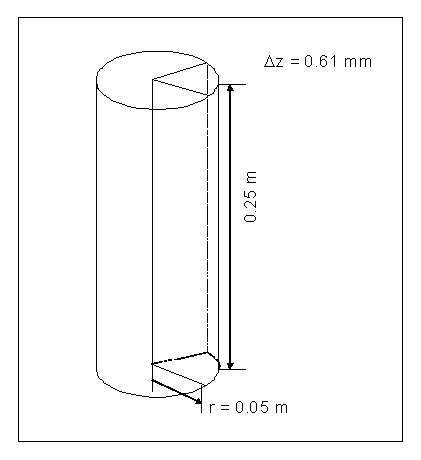
\includegraphics[width=0.4\textwidth]{PART_II/M/fig31.eps}
\caption{Calculation area: a quarter of a cylinder}
\label{Me_fig31}
\end{figure}

\subsubsection{Solution}
\label{subsubsec:Me4_sol}

The calculation area for the threedimensional simulation consists of a quarter of the cylinder under consideration (cf. Fig.~\ref{Me_fig32}). The model includes 4000 elements and 4947 nodes. Deformations in $x$-direction are suppressed in the $y$-$z$-plane and deformations in $y$-direction are suppressed in the $x$-$z$-plane. Furthermore, axial deformations are suppressed at the bottom of the calculation area. At the top of the model boundary conditions are prescribed assuming a constant displacement of 0.61~mm causing compression of the cylinder. The used material parameters are shown in Tab. \ref{Me_tab33}.

\begin{figure}[htbp]
\centering
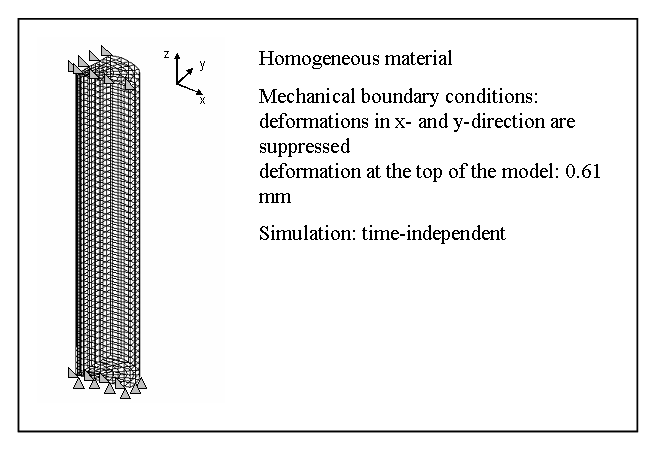
\includegraphics[width=0.65\textwidth]{PART_II/M/fig32.eps}
\caption{Finite element model: spatial discretization and boundary conditions}
\label{Me_fig32}
\end{figure}

\begin{table}[!htb]
\centering
\caption{Material parameters}
\label{Me_tab33}
\begin{tabular}{llll}
\toprule
Symbol & Parameter & Value & Unit \\
\midrule
$E$    & Young's modulus & $7$    & GPa \\
$\nu$  & Poisson's ratio & $0.3$  & -- \\
$\rho$ & Density         & $2500$ & kg$\cdot$m$^{-3}$ \\
\bottomrule
\end{tabular}
\end{table}

In order to solve the homogeneous problem analytically, some constraints have to be considered: the stresses in $x$- and $y$-direction are equal to zero, because the body expands homogeneously in radial direction. Thus the stress-strain equations defined by Hooke's law (\ref{eq:hooke_isotherm}) can be simplified as follows:
\begin{eqnarray}
\varepsilon_{zz} & = &
\frac{\Delta z}{z}\,=\,\frac{1}{E}\cdot\sigma_{zz}
\label{Me_eq36} \\[1.5ex]
\varepsilon_{xx} & = &
\varepsilon_{xx}\,=\,\frac{1}{E}\cdot\left(-\nu\cdot\sigma_{zz}\right)
\label{Me_eq37}
\end{eqnarray}

With the given strain in $z$-direction, the axial stress $\sigma_{zz}$ is defined using Eqn.~\ref{Me_eq36} as
\begin{displaymath}
\frac{\Delta z}{z}\,=\,-2.44\times 10^{-3}
\quad\mathrm{and}\quad
\sigma_{zz}\,=\,-1.71\times 10^{7}\,\mathrm{Pa}
\end{displaymath}

In this way, the strains in $x$- and $y$-direction are known.
\begin{displaymath}
\varepsilon_{xx}\,=\,7.32\times 10^{-4}
\end{displaymath}

\subsubsection{Results}
\label{subsubsec:Me4_res}

As can be seen in Fig.~\ref{Me_fig33}, the numerical results meet exactly the analytical solutions. In this figure, axial strain and the resulting axial stress are presented along a polyline from top to bottom of the calculation area.

\begin{figure}[htbp]
\centering
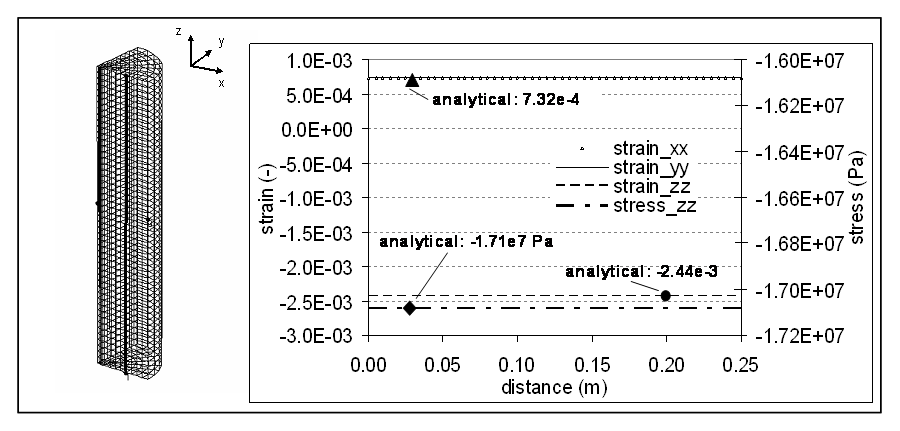
\includegraphics[width=0.9\textwidth]{PART_II/M/fig33.eps}
\caption{Resulting axial straian and axial stress}
\label{Me_fig33}
\end{figure}
